\documentclass[12pt,a4paper]{article}
\usepackage[a4paper,top=1.5cm, bottom=1.5cm, left=1.5cm, right=1.5cm]{geometry}
\usepackage[T2A]{fontenc}
\usepackage[utf8]{inputenc}
\usepackage[russian]{babel}
\usepackage{amsmath}
\usepackage{amssymb}
\usepackage{graphicx}
\usepackage{floatrow}
\usepackage{booktabs}
\usepackage{wrapfig}
\usepackage{indentfirst}
\usepackage{lipsum}
\usepackage{subcaption}
\usepackage{float}
\usepackage{enumitem}
\restylefloat{table}

\newcommand{\figref}[1]{(см. рис. \ref{#1})}
\newcommand{\e}[1]{\text{$\cdot10^{#1}$}}

\author{\normalsize Симанкович Александр, Дедков Денис, Степанов Дмитрий
	\\ \normalsize группа Б01-108 \\
	\normalsize 03.11.2023}
\date{}

\usepackage{float}
\restylefloat{table}
\title{
	\large Отчет о выполнении лабораторной работы \\
	\Large <<Спектры импульсных сигналов>> \\ 
	
}

\begin{document}
\maketitle
\newpage
\section*{5.1. Последовательность радиоимпульсов.}
\subsection*{Перемычка П5 *выключена*}
\vspace*{20pt}

\begin{center}
	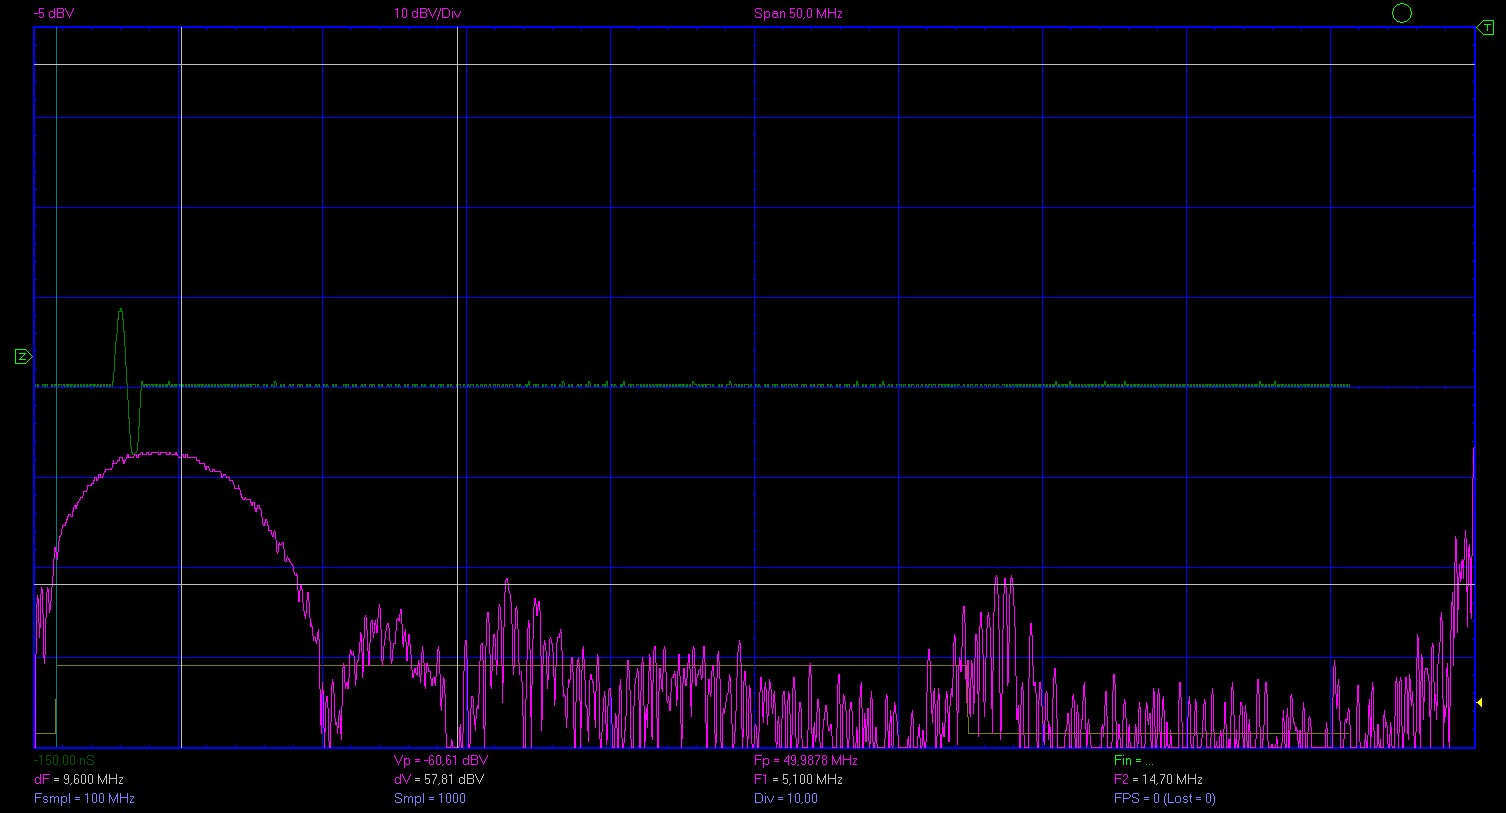
\includegraphics[width=.8\linewidth]{data/51_n1_nop5}\hfill
\end{center}	
\begin{center}
	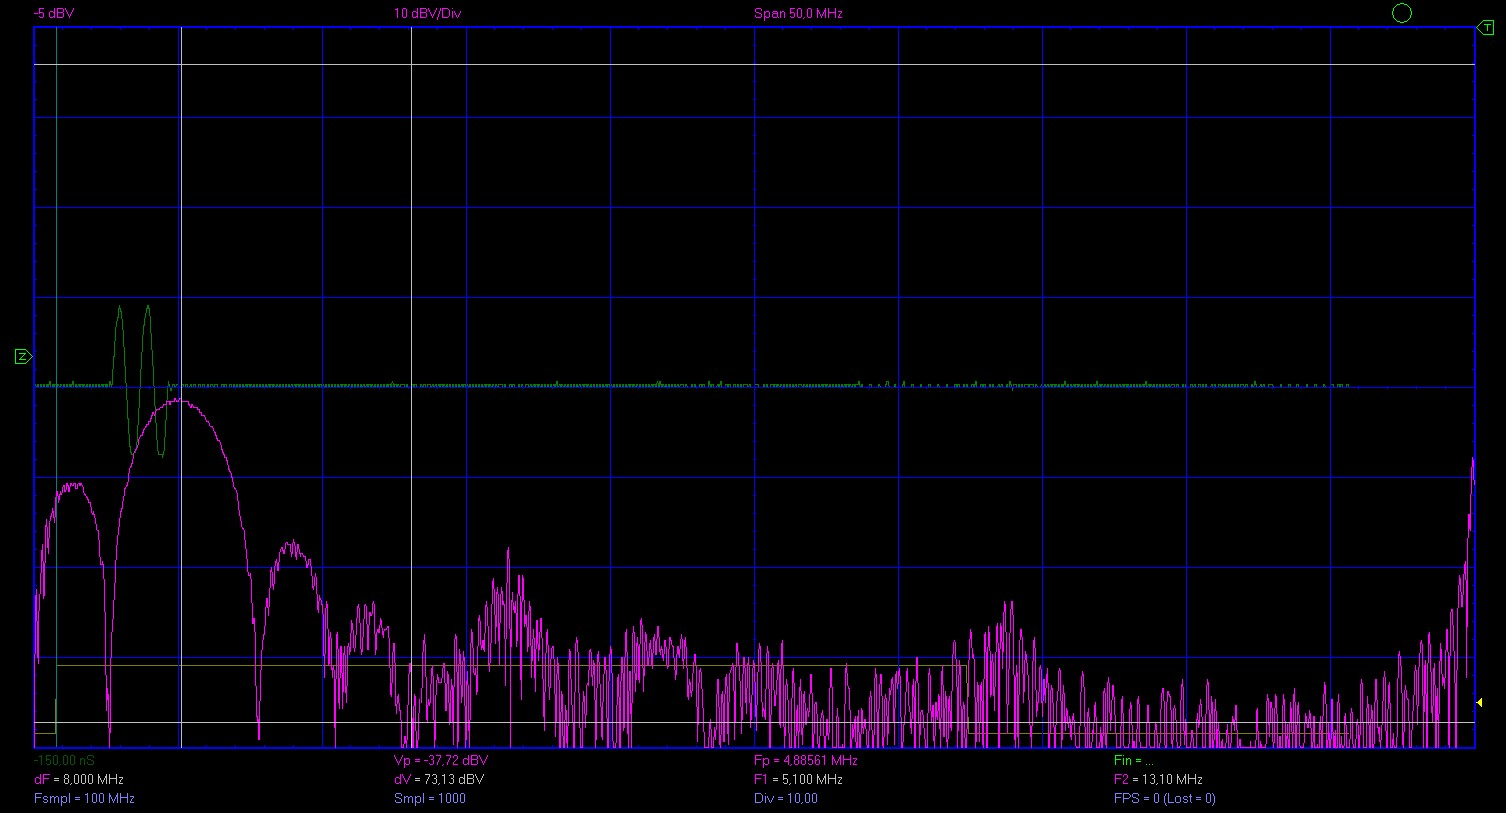
\includegraphics[width=.8\linewidth]{data/51_n2_nop5}\hfill
\end{center}	
\begin{center}
	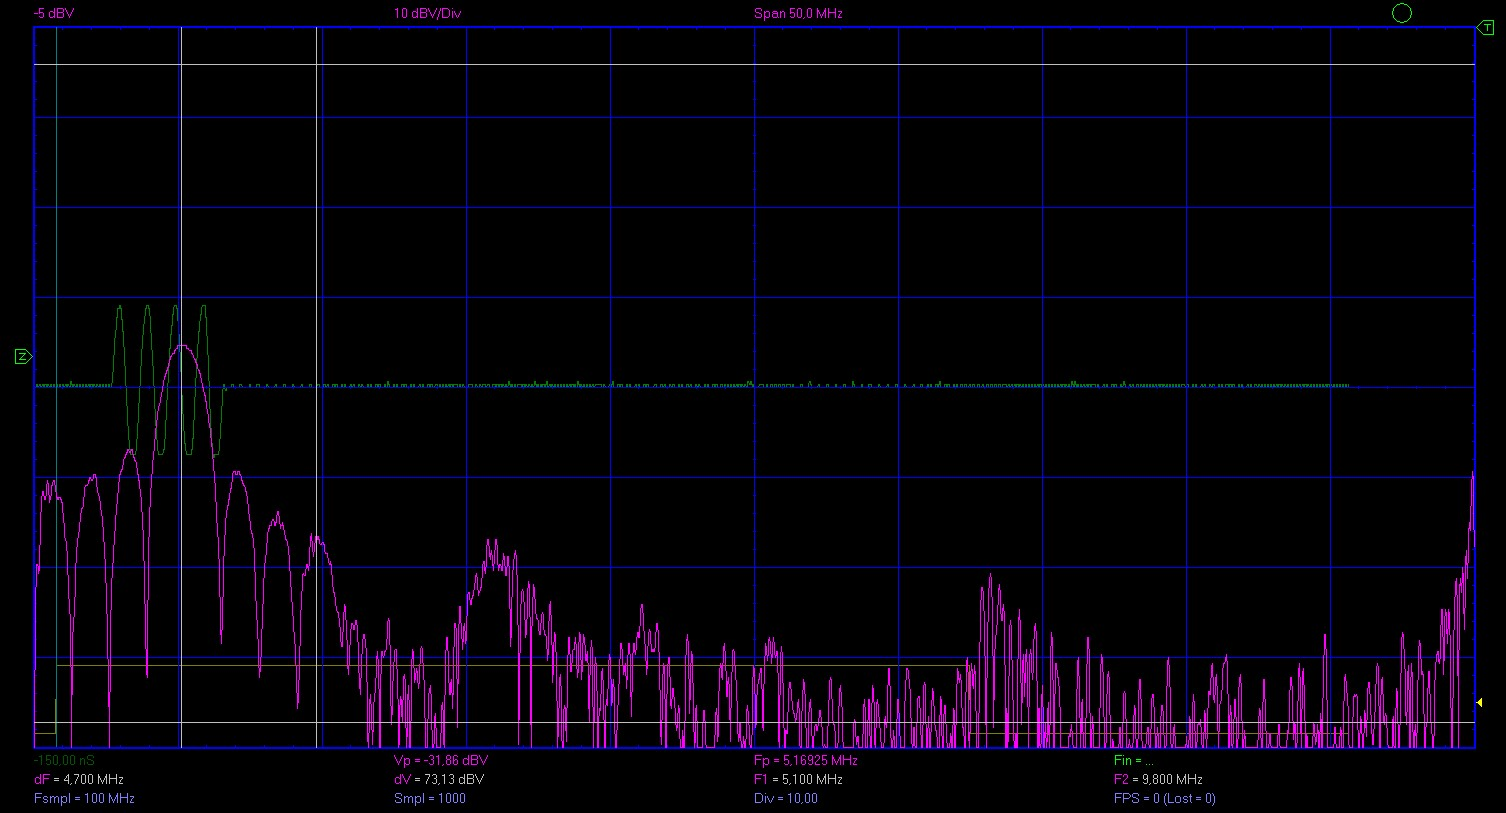
\includegraphics[width=.8\linewidth]{data/51_n4_nop5}\hfill
\end{center}	

\subsection*{Перемычка П5 *включена*}
\begin{center}
	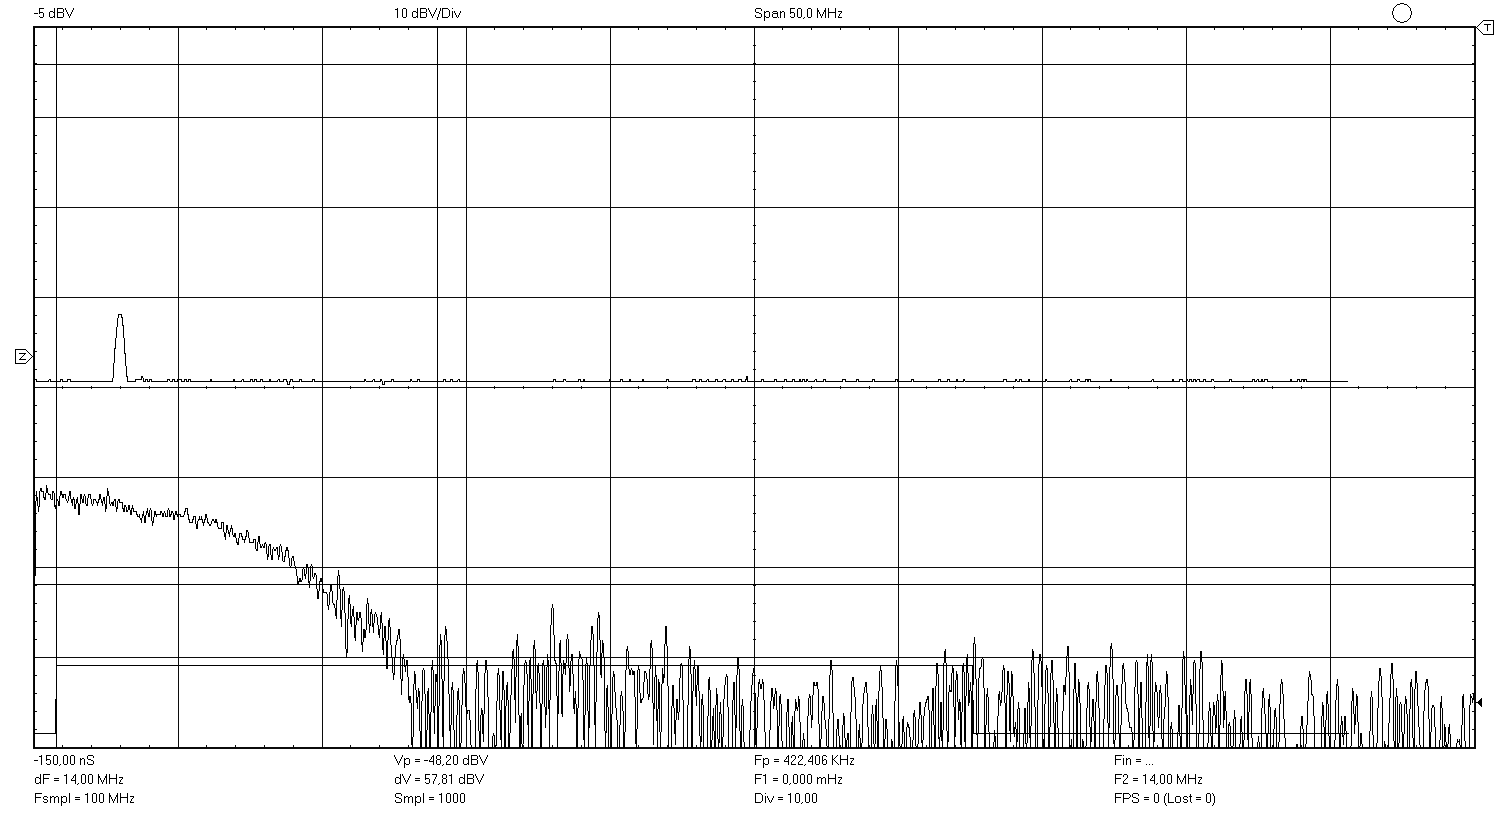
\includegraphics[width=.8\linewidth]{data/51_n1_p5}\hfill
\end{center}	
\begin{center}
	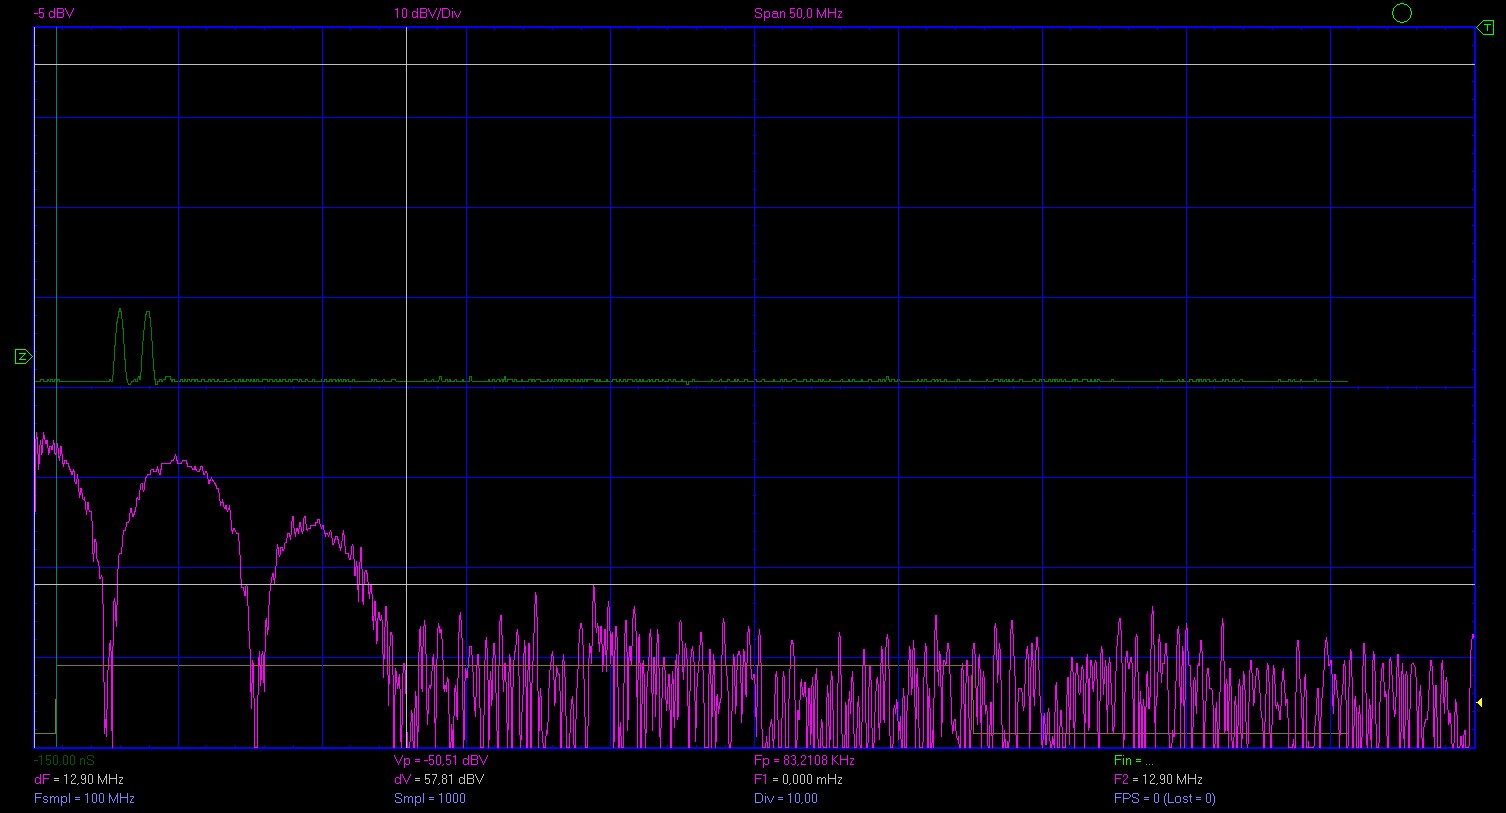
\includegraphics[width=.8\linewidth]{data/51_n2_p5}\hfill
\end{center}	
\begin{center}
	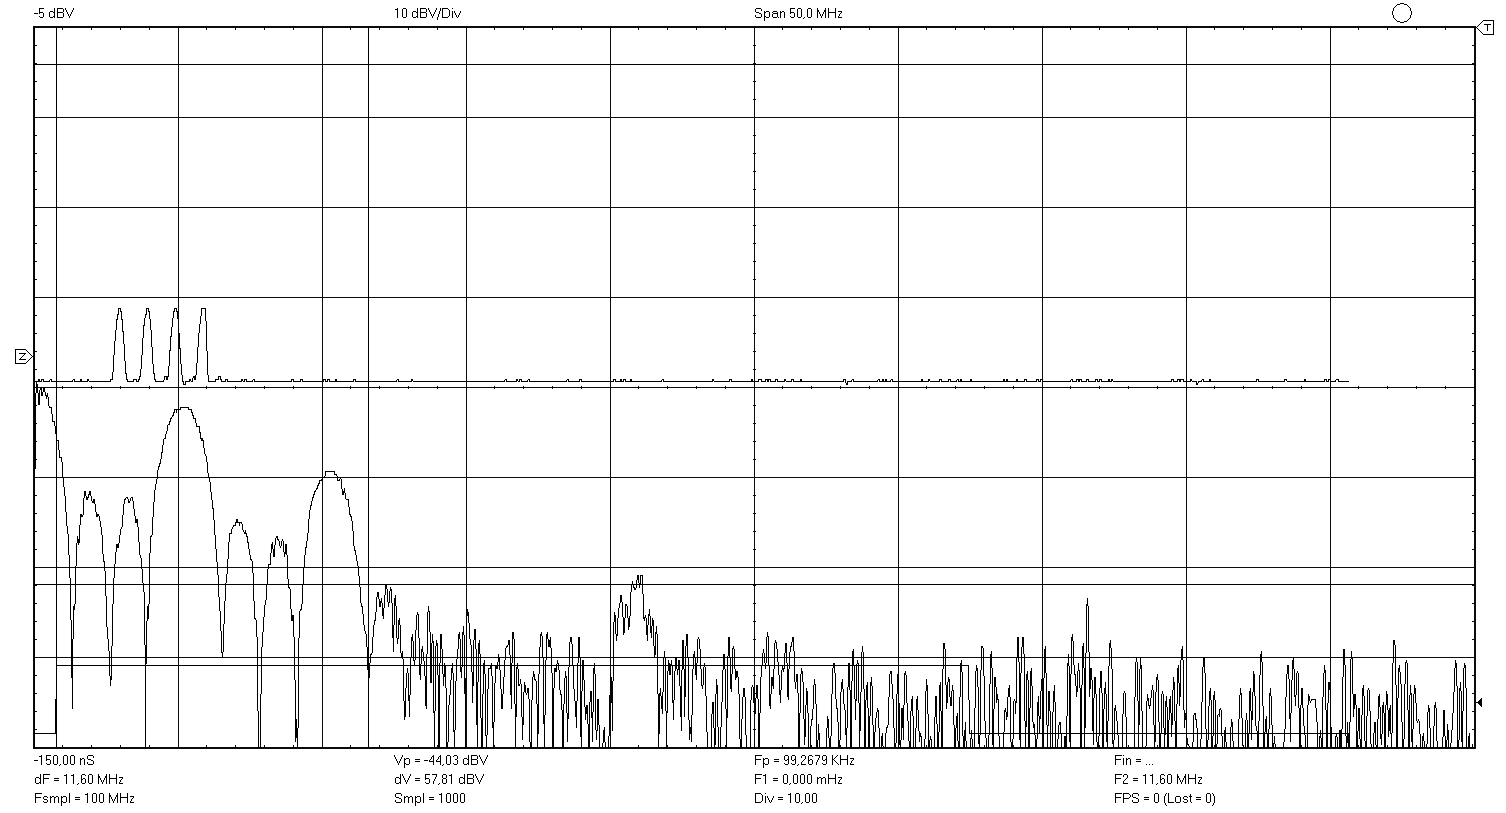
\includegraphics[width=.8\linewidth]{data/51_n4_p5}\hfill
\end{center}	

\subsection*{5.2. Последовательность прямоугольных импульсов.}
\vspace*{20pt}

\subsection*{Перемычка П1 *неинвертирован*}
\begin{center}
	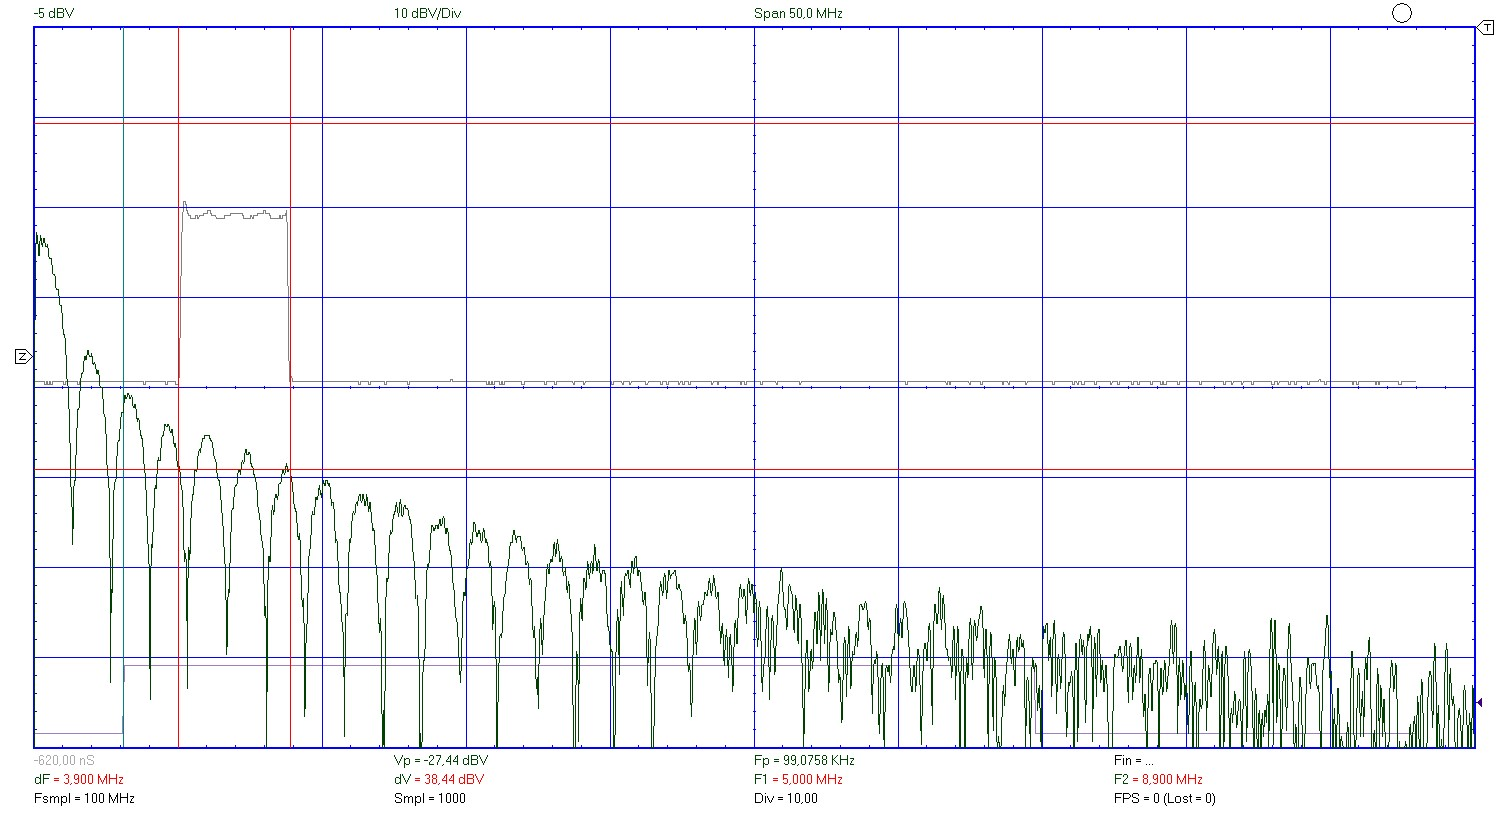
\includegraphics[width=.8\linewidth]{data/52}\hfill
\end{center}	
\subsection*{Перемычка П1 *инвертирован*}
\begin{center}
	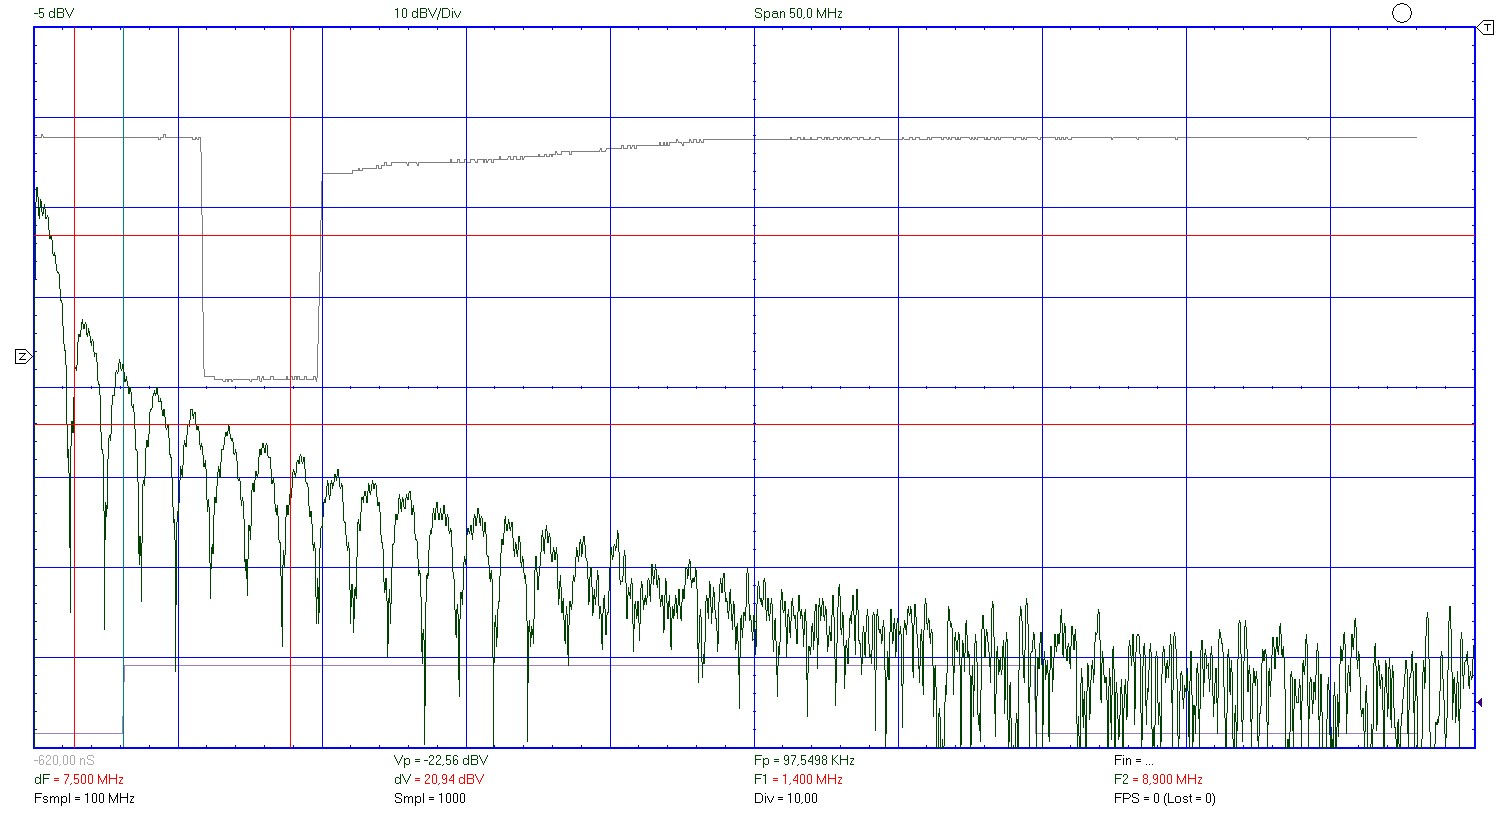
\includegraphics[width=.8\linewidth]{data/52_inv}\hfill
\end{center}	
\newpage

\subsection*{5.3. Последовательность пачек прямоугольных импульсов.}
\vspace*{20pt}

\begin{center}
	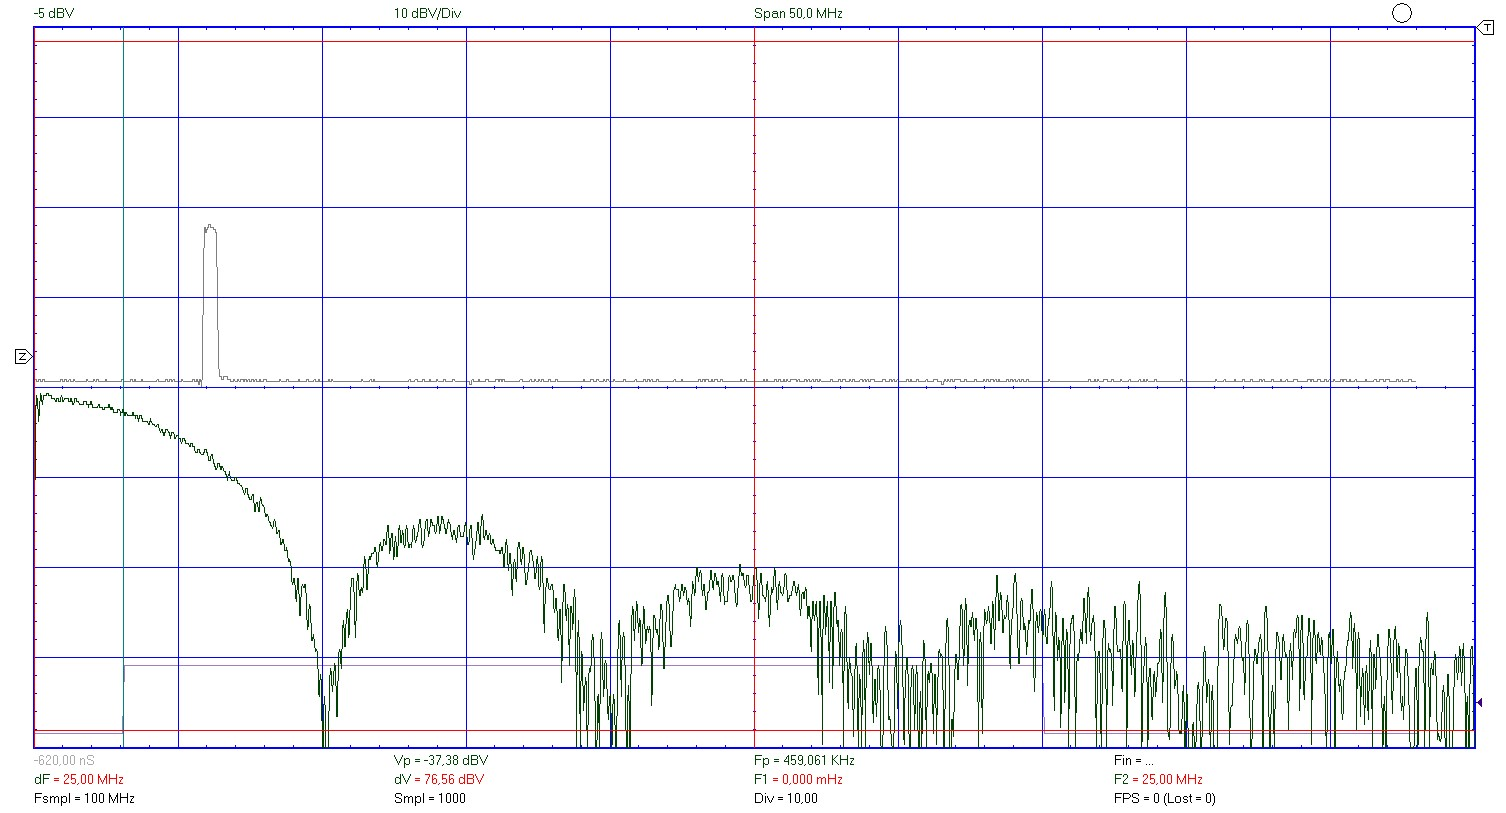
\includegraphics[width=.8\linewidth]{data/53_n1}\hfill
\end{center}	
\begin{center}
	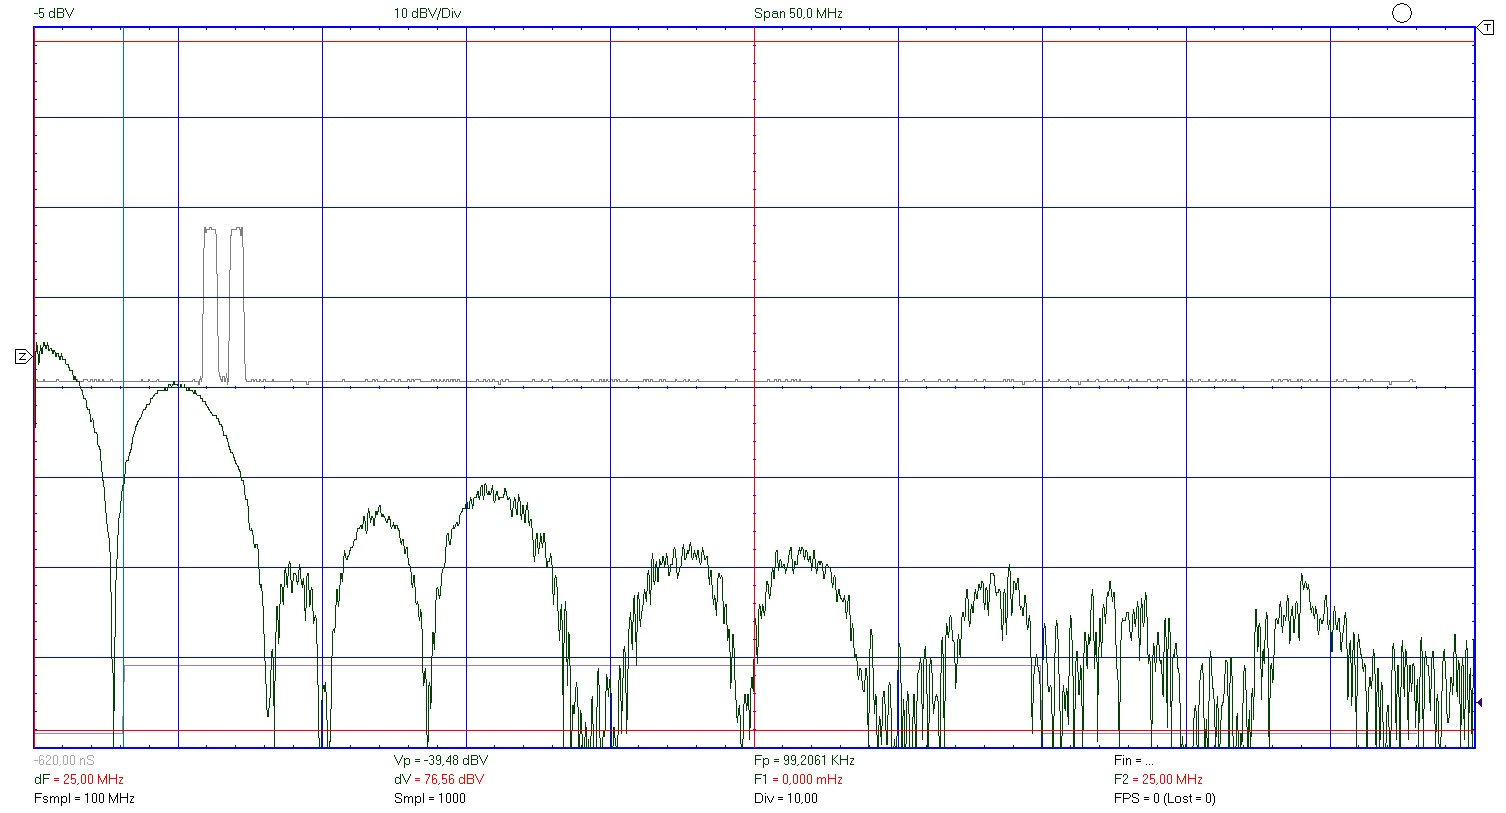
\includegraphics[width=.8\linewidth]{data/53_n2}\hfill
\end{center}	
\begin{center}
	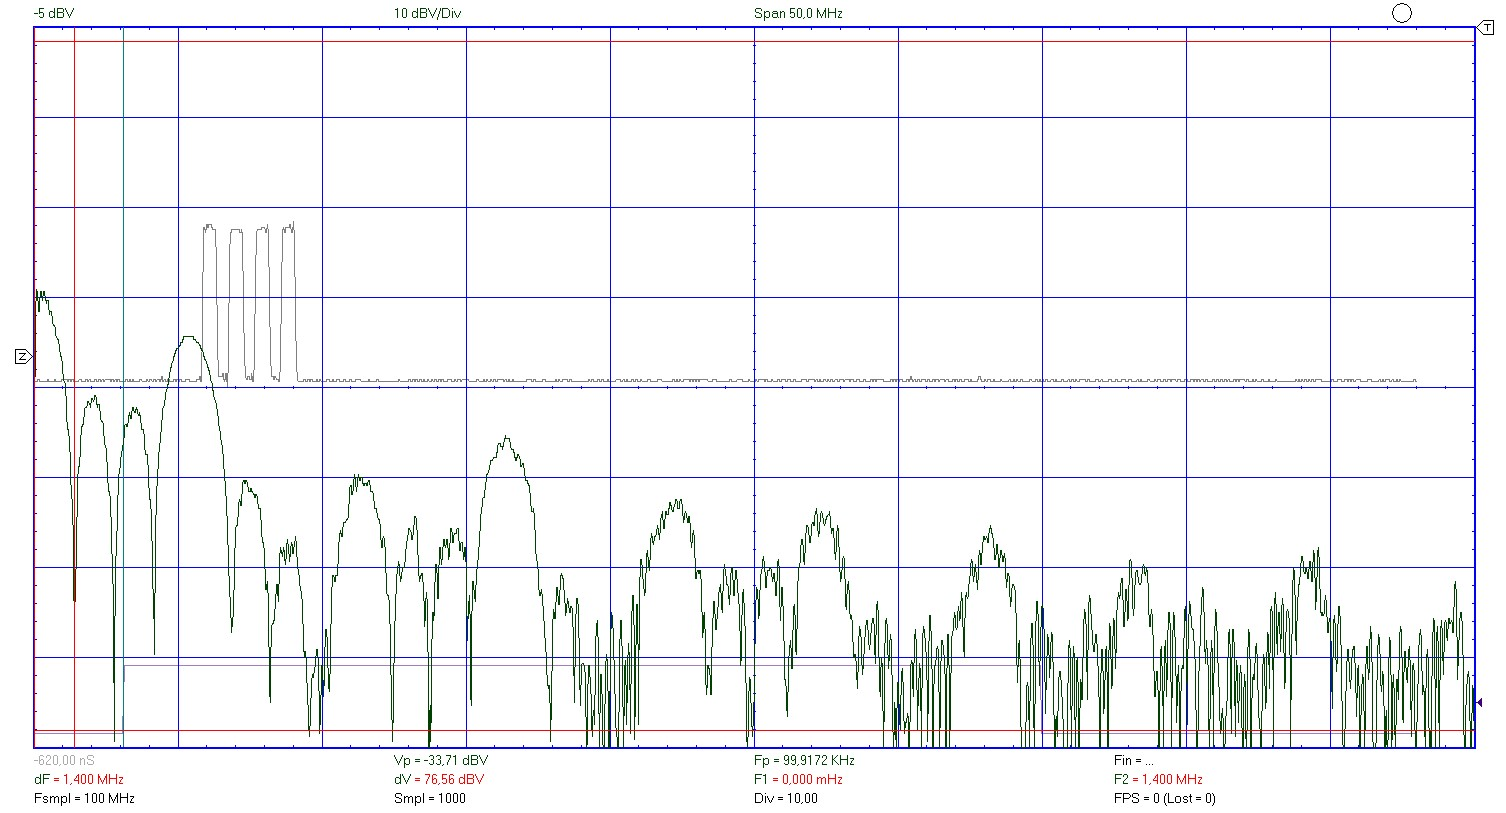
\includegraphics[width=.8\linewidth]{data/53_n4}\hfill
\end{center}	

\newpage

\subsection*{5.4. Последовательность коротких импульсов.}
\vspace*{20pt}

\begin{center}
	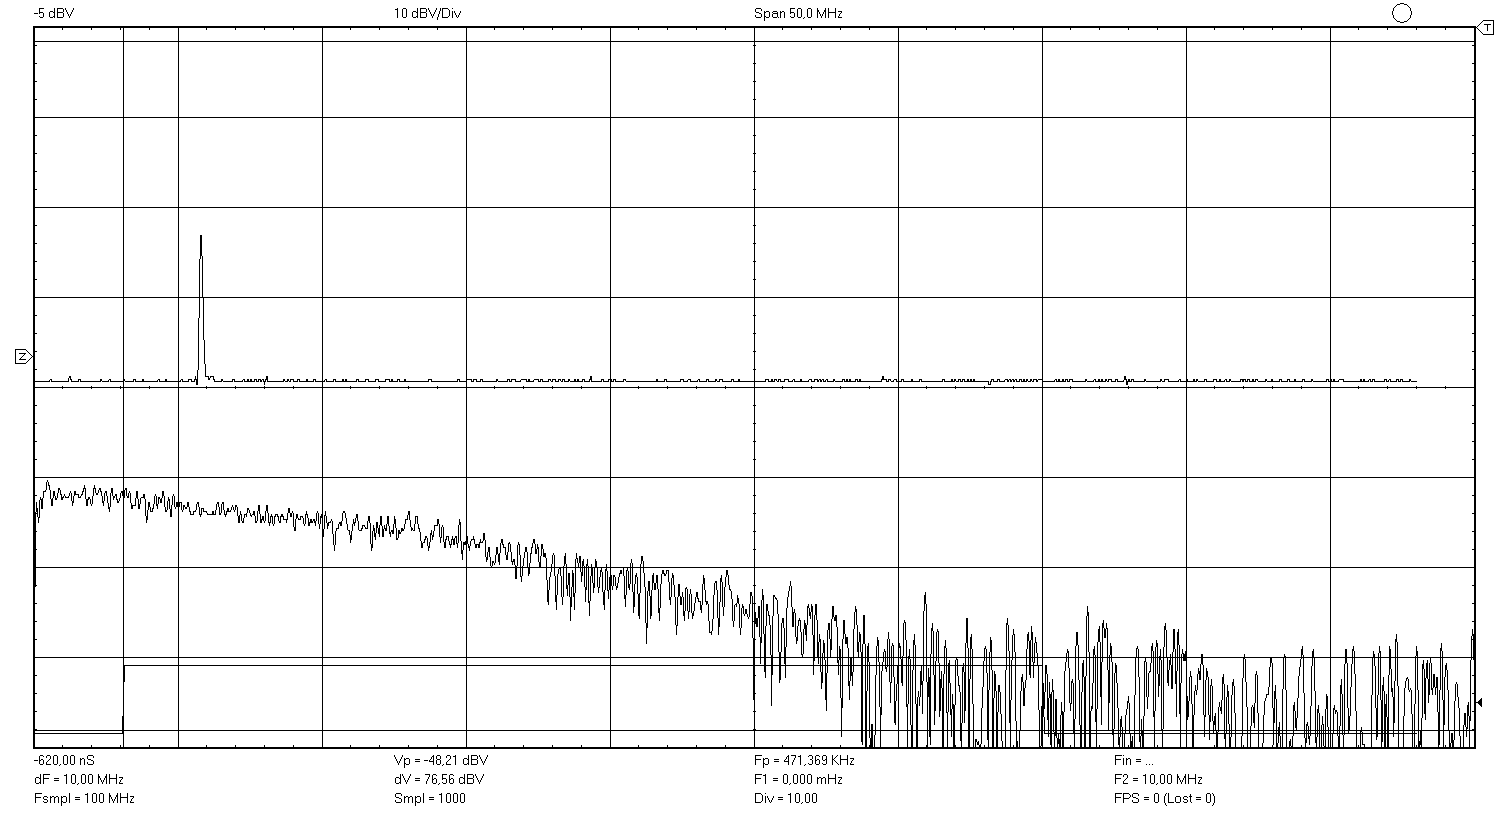
\includegraphics[width=.8\linewidth]{data/54_kt3}\hfill
\end{center}	
\begin{center}
	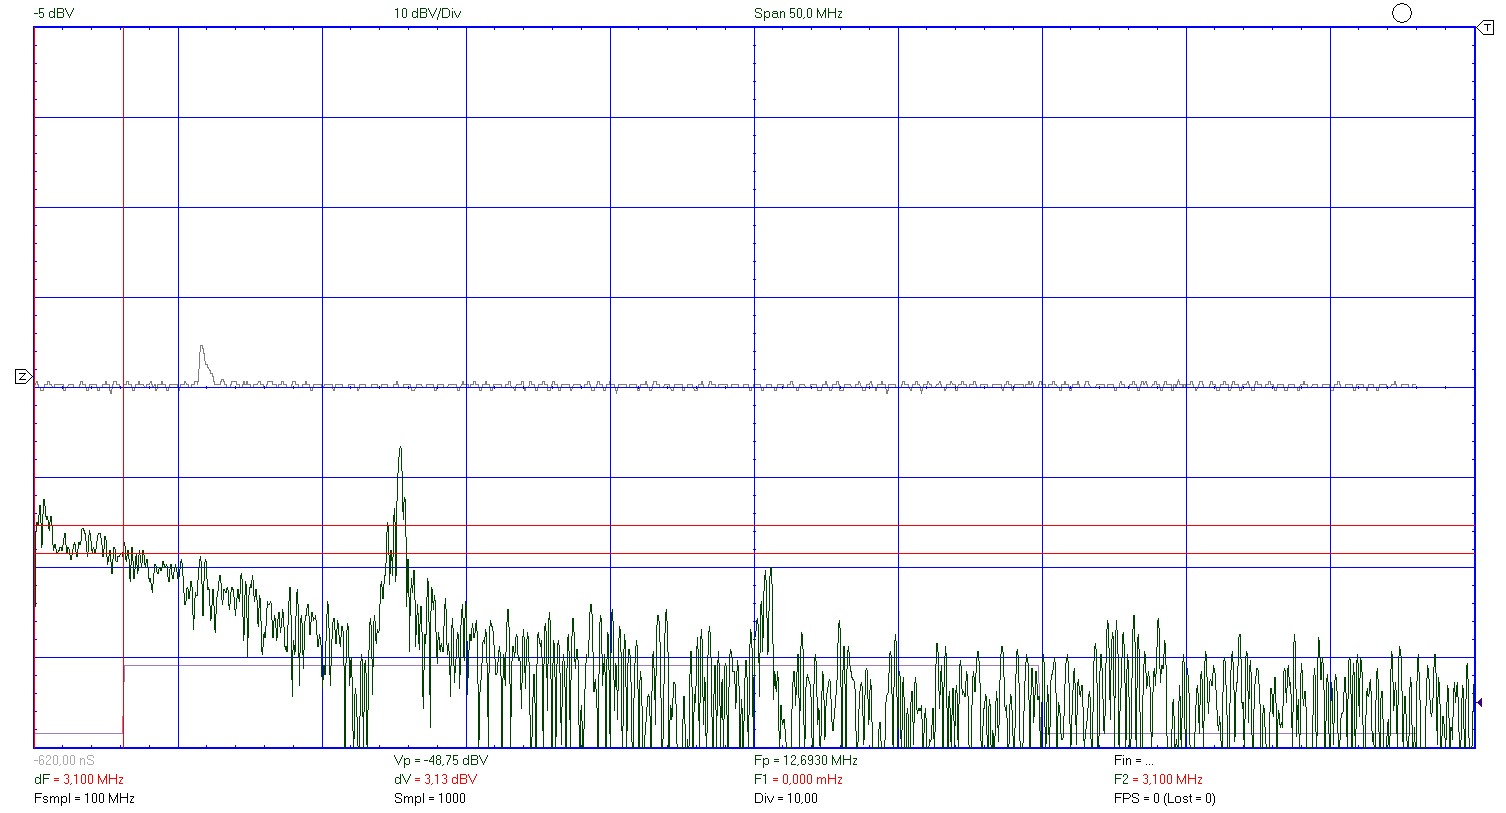
\includegraphics[width=.8\linewidth]{data/54_kt4}\hfill
\end{center}	
\begin{center}
	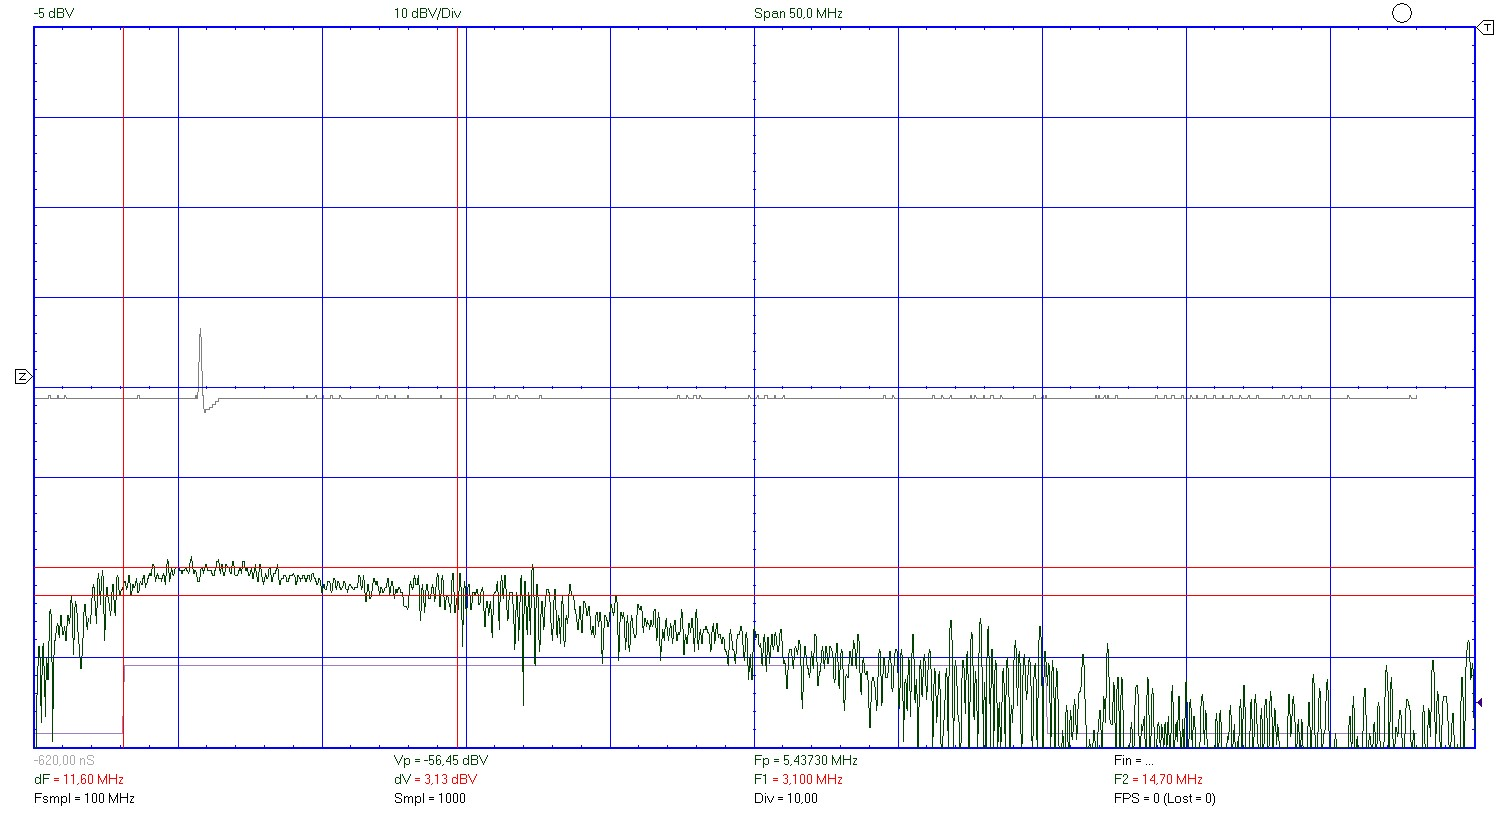
\includegraphics[width=.8\linewidth]{data/54_kt5}\hfill
\end{center}	

\newpage


\end{document}
